\documentclass[a4paper,12pt]{article}
\usepackage{amsmath,amsfonts,amsthm,amssymb}
\usepackage{physics}
\usepackage{geometry}
\usepackage{graphicx}
\usepackage{setspace}

\author{Gordon Chan}
\title{Solution for The Pure Mathematics Portion of 2020 GCE `A' Levels Mathematics Paper 2}

\begin{document}
\maketitle

\section*{1}
Let the curve be \(y=ax^2+bx+c\).
\[(1,-2)\implies a+b+c=-2\]
\[\begin{aligned}
    y^\prime&=2ax+b\\
    y^\prime(1)&=0\implies2a+b=0\\
    y^\prime(2)&=5\implies 4a+b=5
\end{aligned}\]
\[\begin{cases}
    a+b+c=-2\\
    2a+b=0\\
    4a+b=5
\end{cases}
\implies
\begin{cases}
    a=\frac52\\
    b=-5\\
    c=\frac12
\end{cases}\]
\[\therefore\boxed{y=\frac52x^2-5x+\frac12}\]

\section*{2}
\subsection*{(a)}
\subsubsection*{(i) (A)}
The sequence increases indefinitely and diverges to positive infinity.
\subsubsection*{(i) (B)}
The sequence stays constant at 5.
\subsubsection*{(ii)}
\[\begin{aligned}
    u_5&=2u_4-5\\
       &=2(2u_3-5)-5\\
       &=4u_3-15\\
       &=4(2u_2-5)-15\\
       &=8u_2-35\\
       &=8(2u_1-5)-35\\
       &=16p-75\\
\end{aligned}\]
\[u_5=101\implies 16p-75=101\implies p=\boxed{11}\]
\subsection*{(b)}
\subsubsection*{(i)}
\[\begin{aligned}
    v_4&=v_4\\
    b+2v_3-7&=2v_3\\
    b-7&=0\\
    b&=\boxed7
\end{aligned}\]
\subsubsection*{(ii)}
\[\begin{aligned}
    v_5&=v_3+2v_4-7\\
       &=v_3+4v_3-7\\
       &=5v_3-7\\
       &=5(a+2b-7)-7\\
       &=5(a+14-7)-7\\
       &=5(a+7)-7\\
       &=5a+35-7\\
       &=\boxed{5a+28}\\
\end{aligned}\]
\subsection*{(c)}
\subsubsection*{(i)}
\[\begin{aligned}
    \sum_{r=1}^n{a_r}&=a_n+\sum_{r=1}^{n-1}{a_r}\\
    a_n&=\sum_{r=1}^n{a_r}-\sum_{r=1}^{n-1}{a_r}\\
      &=n^3-11n^2+4n-\pqty{{(n-1)}^3-11{(n-1)}^2+4(n-1)n}\\
      &=n^3-11n^2+4n-\pqty{n^3-3n^2+3n-1-11\pqty{n^2-2n+1}+4n-4}\\
      &=n^3-11n^2+4n-\pqty{n^3-3n^2+7n-5-11n^2+22n-11}\\
      &=n^3-11n^2+4n-\pqty{n^3-14n^2+29n-16}\\
      &=n^3-11n^2+4n-n^3+14n^2-29n+16\\
      &=\boxed{3n^2-25n+16}
\end{aligned}\]
\subsubsection*{(ii)}
\[\begin{aligned}
    \sum_{r=1}^m{a_r}&=\sum_{r=1}^3{a_r}\\
    m^3-11m^2+4m&=3^3-11{(3)}^2+4(3)\\
    m^3-11m^2+4m+60&=0\\
    (m-3)\left(m^2-8m-20\right)&=0\\
    (m-3)(m+2)(m-10)&=0\\
    m-10&=0\\
    m&=\boxed{10}
\end{aligned}\]

\section*{3}
\subsection*{(i)}
\[x=3t^2+2\implies\dv{x}{t}=6t\]
\[y=6t-1\implies\dv{y}{t}=6\]
\[\dv{y}{x}=\frac{\dv{y}{t}}{\dv{x}{t}}=\frac6{6t}=\frac1t\]
At \((x_0,y_0)=(14,11)\), \(y_0=11\implies11=6t_0-1\implies t_0=2\).
\[m=\eval{\dv{y}{x}}_{t=t_o}=\frac1{t_0}=\frac12\]
\[\begin{aligned}
    y-y_0&=-\frac1m(x-x_0)\\
    y-11&=-2(x-14)\\
    y-11&=-2x+28
\end{aligned}\]
\[N:\boxed{2x+y=39}\]
\[a=\boxed2,b=\boxed1,c=\boxed{39}\]
\subsection*{(ii)}
\begin{center}
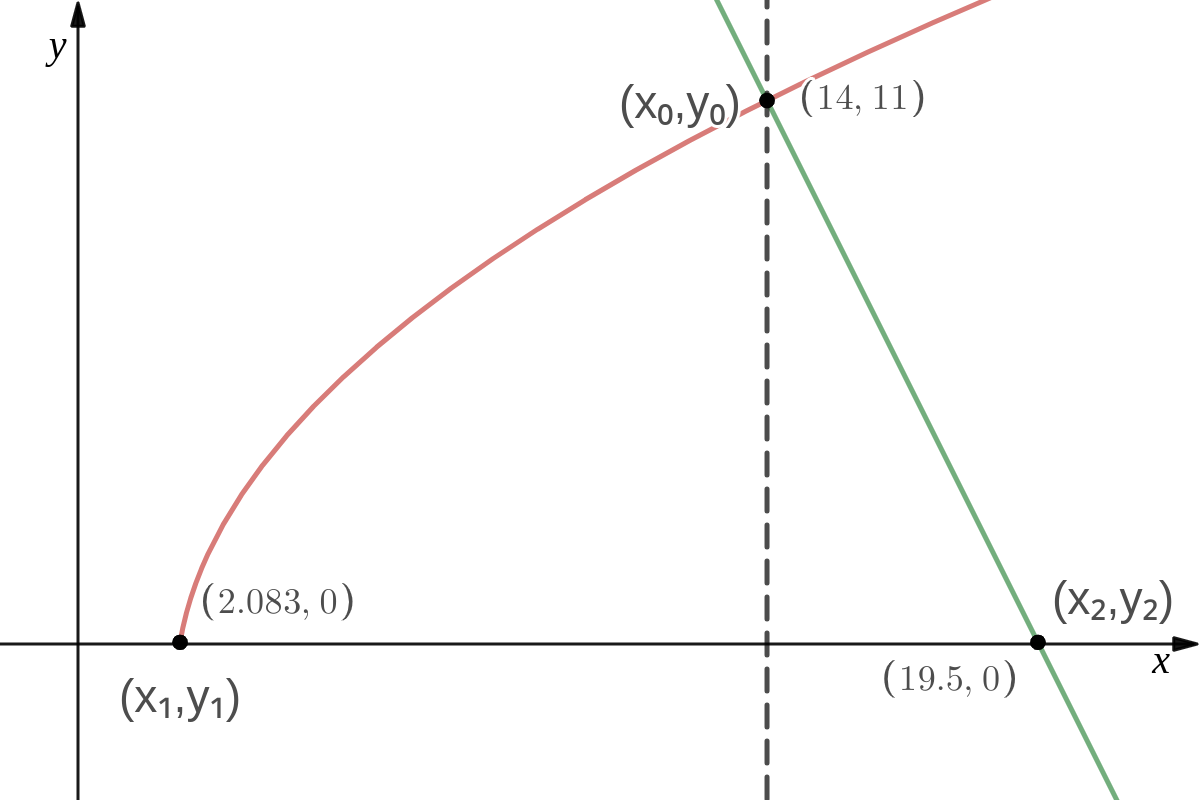
\includegraphics[width=.69\textwidth]{q3.png}
\end{center}
\[\begin{aligned}
    y_1&=0\\
    6t_1-1&=0\\
    6t_1&=1\\
    t_1&=\frac16\\
    x_1&=3\pqty{\frac16}^2+2\\
    x_1&=\frac{25}{12}
\end{aligned}\]
\[\begin{aligned}
    y_2&=0\\
    2x_2+0&=39\\
    x_2&=\frac{39}2
\end{aligned}\]
\[\begin{aligned}
    A&=\int_{x_1}^{x_0}y\dd{x}+\frac12(x_2-x_0)y_0\\
     &=\int_{t_1}^{t_0}y\dv{x}{t}\dd{t}+\frac12(x_2-x_0)y_0\\
     &=\int_{\frac16}^2(6t-1)(6t)\dd{t}+\frac12\left(\frac{39}2-14\right)(11)\\
     &=6\int_{\frac16}^2\pqty{6t^2-t}\dd{t}+\frac{121}4\\
     &=6\eval{\pqty{2t^3-\frac12t^2}}_{\frac16}^2+\frac{121}4\\
     &=6\pqty{14-\pqty{-\frac1{216}}}+\frac{121}4\\
     &=6\pqty{\frac{3025}{216}}+\frac{121}4\\
     &=\frac{3025}{36}+\frac{121}4\\
     &=\boxed{\frac{2057}{18}\,\text{units}^2}
\end{aligned}\]
\subsection*{(iii)}
\subsubsection*{(a)}
\[A^\prime=(2\times3)A=6\pqty{\frac{2057}{18}}=\boxed{\frac{2057}3\,\text{units}^2}\]
\subsubsection*{(b)}
\[C:\begin{cases}
    x=3t^2+2\\
    y=6t-1
\end{cases}
,\,t\geqslant\frac16\]
\[x=3t^2+2\implies t=\sqrt{\frac{x-2}3}\quad(t\geqslant0)\]
\[t\geqslant\frac16\implies x\geqslant\frac{25}{12}\]
\[\begin{aligned}
    y&=6t-1\\
    C:y&=6\sqrt{\frac{x-2}3}-1,\,x\geqslant\frac{25}{12}
\end{aligned}\]
\[C\to D\implies (x,y)\to\pqty{\frac x2,\frac y3}\]
\[\frac x2\geqslant\frac{25}{12}\implies x\geqslant\frac{25}6\]
\[\frac y3=6\sqrt{\frac{\frac x2-2}3}-1\]
\[\therefore D:\boxed{y=18\sqrt{\frac{x-4}6}-3,\,x\geqslant\frac{25}6}\]

\section*{4}
\subsection*{(i)}
\[h+a+h=30\implies h=\frac{30-a}2\]
\[\begin{aligned}
    H^2+\pqty{\frac a2}^2&=h^2\\
    H^2&=\pqty{\frac{30-a}2}^2-\pqty{\frac a2}^2\\
       &=\frac{900-60a+a^2}4-\frac{a^2}4\\
       &=225-15a\qed
\end{aligned}\]
\subsection*{(ii)}
\[\begin{aligned}
    V&=\frac13a^2H\\
     &=\frac13\sqrt{a^4}\sqrt{225-15a}\\
    V&=\frac{\sqrt{225a^4-15a^5}}3\\
    \dv{V}{a}&=\frac{900a^3-75a^4}{6\sqrt{225a^4-15a^5}}\\
\end{aligned}\]
\[\begin{aligned}
    \dv{V}{a}&=0\\
    900a^3-75a^4&=0\\
    900-75a&=0\\
    a&=12
\end{aligned}\]
\[V_{\max}=\frac13\pqty{12}^2\sqrt{225-15(12)}=\boxed{144\sqrt5\,\text{cm}}\]
\subsection*{(iii)}
\[\begin{aligned}
    A&=4\pqty{\frac12ah}\\
     &=2a\pqty{\frac{30-a}2}\\
    A&=30a-a^2\\
    \dv{A}{a}&=30-2a
\end{aligned}\]
\[\begin{aligned}
    \dv{A}{a}&=0\\
    30-2a&=0\\
    a&=\boxed{15}
\end{aligned}\]
\subsection*{(iv)}
The shape formed from the net in this case is a square with side lenth of \(15\sqrt2\,\text{cm}\).
\end{document}
